While vector databases excel at semantic similarity search, graph databases are optimized for managing and querying data with intricate and meaningful relationships. In a graph database, data entities are represented as nodes (or vertices) and the relationships between them as edges. This model is exceptionally well-suited for the domain of \aclp{rs}, where the ecosystem of users, items, and interactions can be naturally represented as a graph.

Modeling data in this way allows for powerful and intuitive querying of complex relationships. For example, collaborative filtering can be implemented by traversing the graph to find users who have rated the same items, and explanations for recommendations can be generated by identifying the paths that connect a user to a suggested item.

This project relies on FalkorDB \cite{FALKORDB}, a high-performance knowledge graph database built on Redis, which uses sparse matrices and linear algebra to accelerate graph operations. It serves as the primary data store for user-item interactions, enabling efficient graph-based recommendation and explanation generation, which are central to the system's functionality. Graphs created using FalkorDB may be managed through the FalkorDB Browser application, as illustrated in Figure~\ref{FIG:FALKORDB_BROWSER}.

\begin{figure}[FalkorDB Browser Interface]{FIG:FALKORDB_BROWSER}{FalkorDB Browser Interface.}
    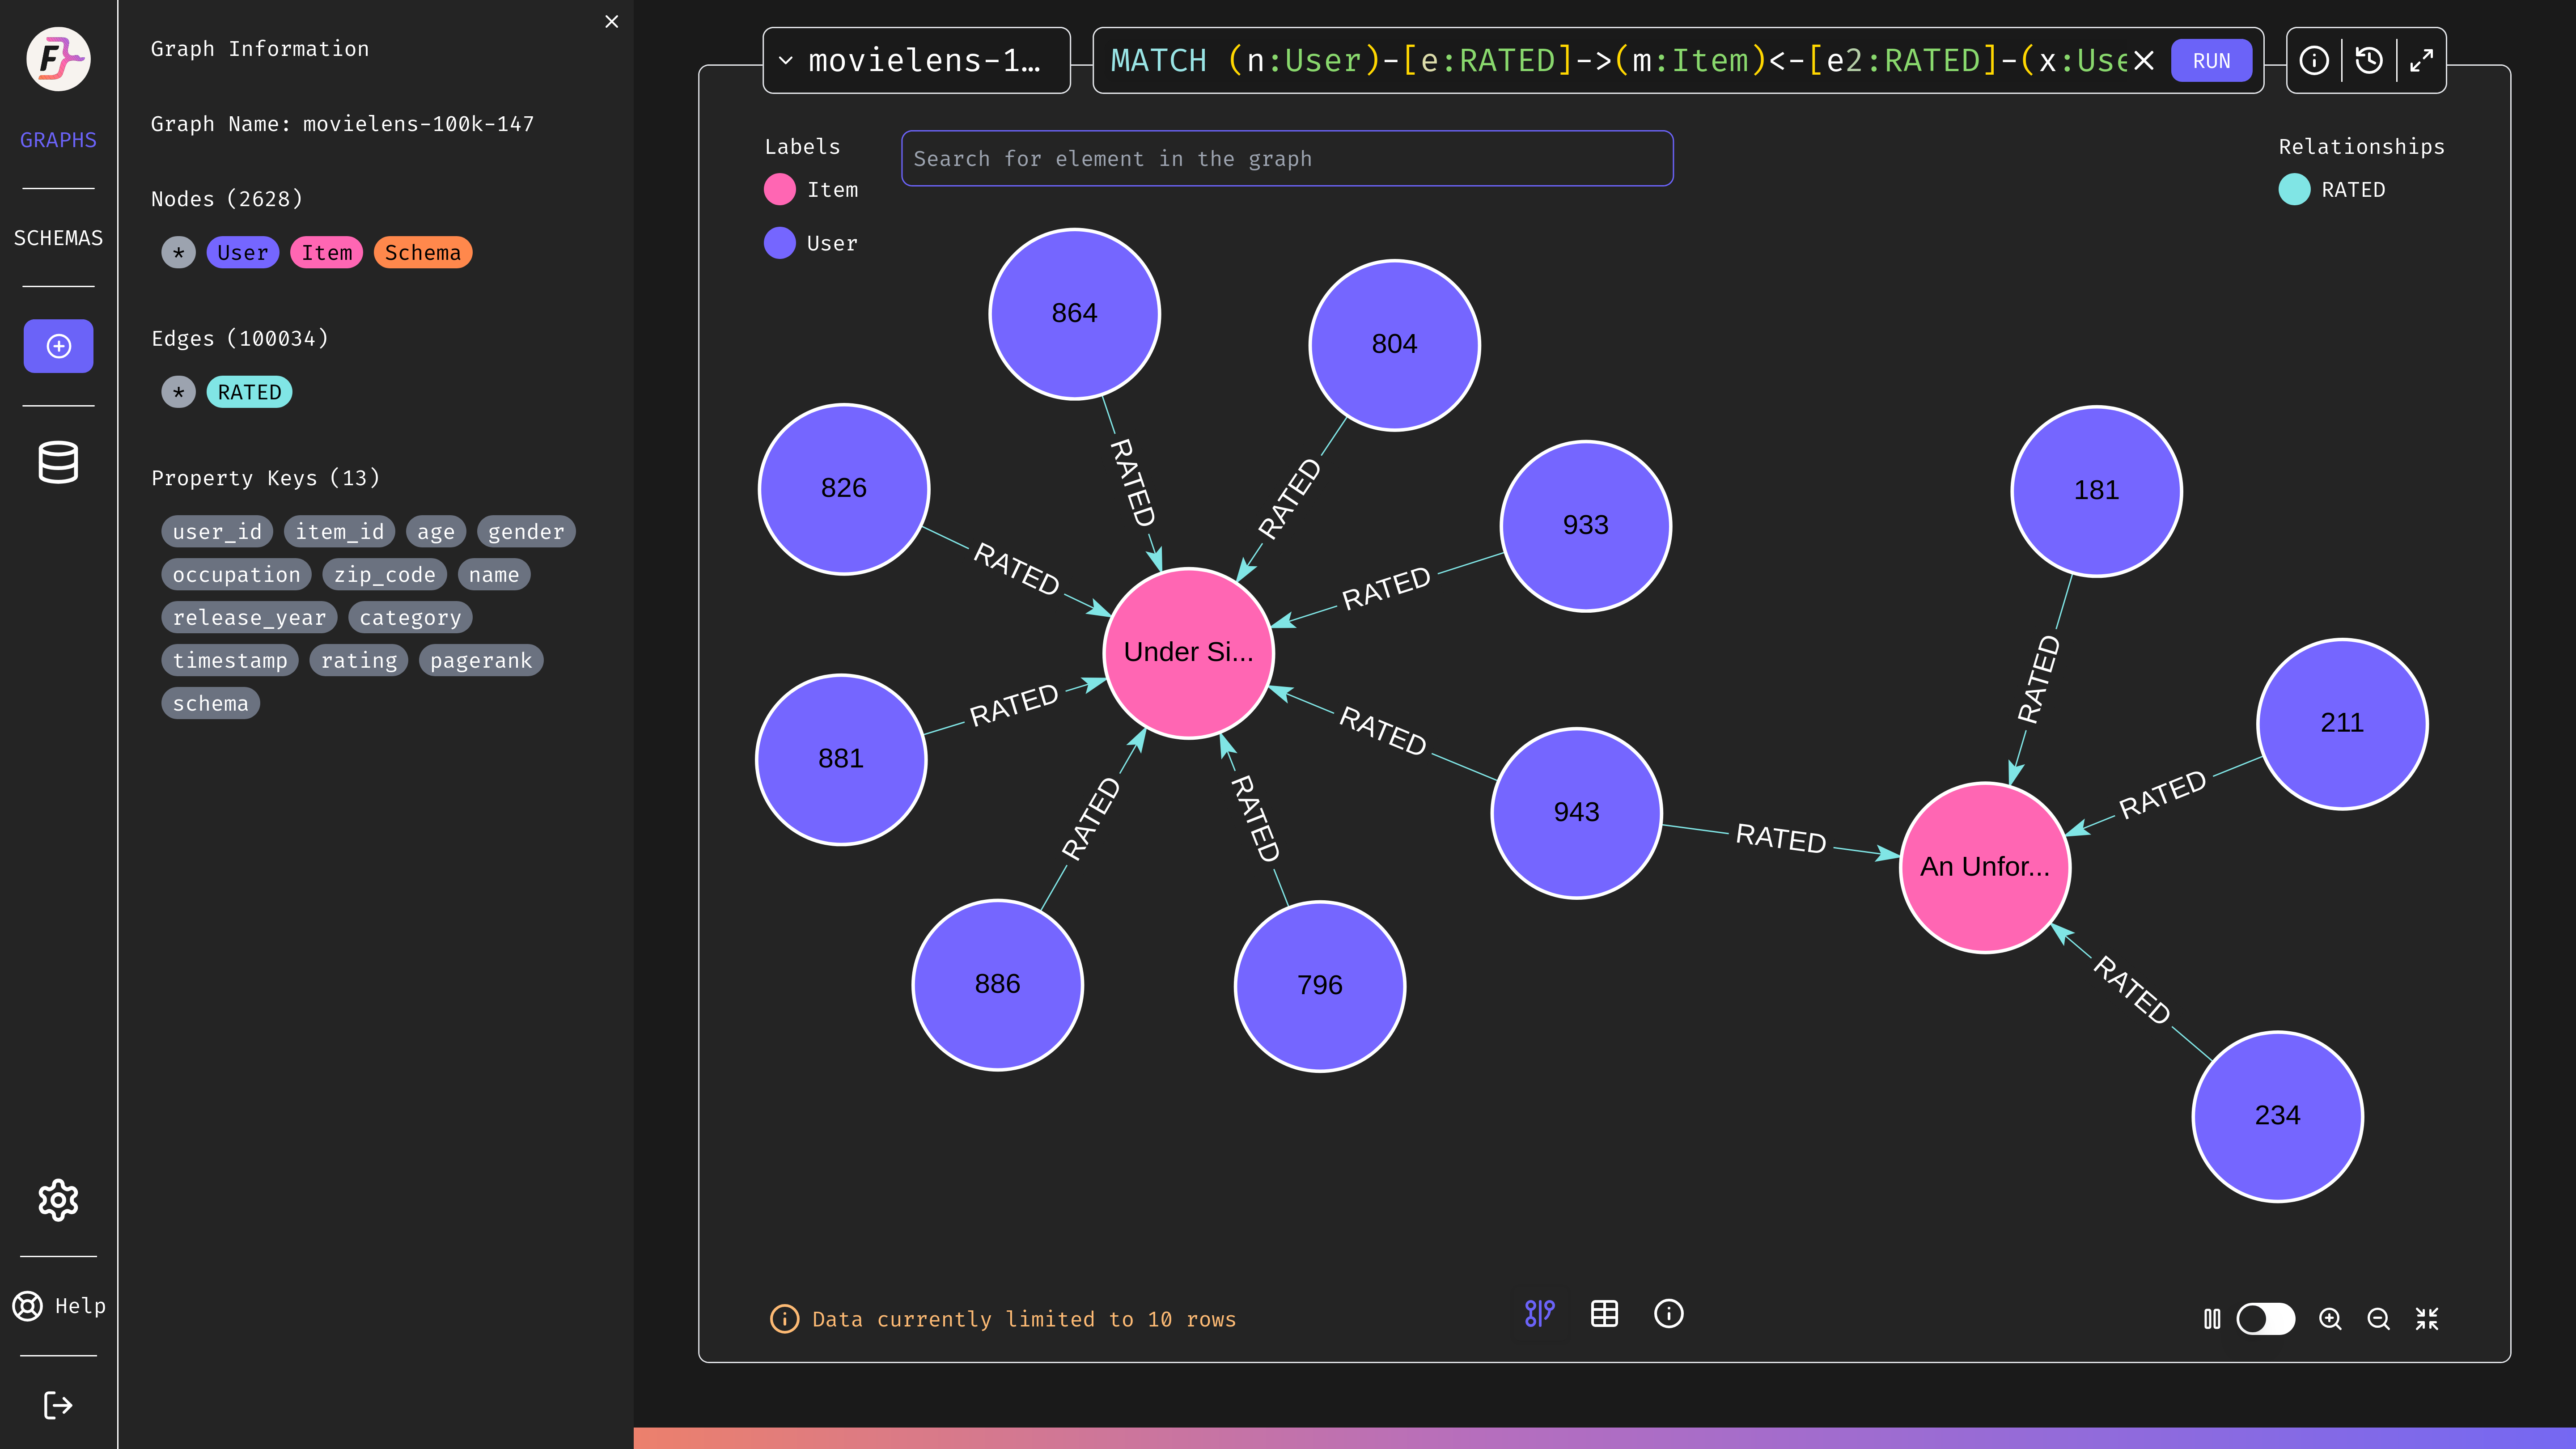
\includegraphics[width=\textwidth]{screenshots/falkordb_browser.png}
\end{figure}
